\RequirePackage[l2tabu, orthodox]{nag}
\documentclass[11pt,chapterprefix=true,toc=bibliography,numbers=noendperiod,
               footnotes=multiple,twoside]{scrreprt}
\usepackage{fixltx2e} % LaTeX patches, \textsubscript
\usepackage{microtype}
\usepackage{cmap} % fix search and cut-and-paste in Acrobat
\usepackage{ifthen}
\usepackage[oldstylenums,largesmallcaps]{kpfonts}
\usepackage[T1]{fontenc}
\usepackage[utf8]{inputenc}
\usepackage[british]{babel}
\usepackage[table,hyperref,dvipsnames]{xcolor}
\usepackage{floatrow}
\usepackage{csquotes}
\usepackage{tabularx}
\usepackage{graphicx}
\usepackage{booktabs}
\usepackage{algorithmicx}
\usepackage{algpseudocode}
\usepackage{algorithm}
\usepackage{mathtools}
\usepackage[chapter]{minted}
\usepackage{caption}
\usepackage{subcaption}
\usepackage{paralist}
\usepackage[autocite=footnote,citestyle=authoryear-comp,bibstyle=authoryear,
            isbn=false,doi=false,backend=biber]{biblatex}
\usepackage[hidelinks]{hyperref}

% TODO: list of figures, algorithms, tables?
% TODO: custom cover page?

%%% Custom LaTeX preamble
% serif, non-bold headings:
\addtokomafont{chapter}{\mdseries}
\addtokomafont{disposition}{\rmfamily}
\addtokomafont{descriptionlabel}{\rmfamily}
\addtokomafont{pageheadfoot}{\itshape}
% section numbering up to subsection
\setcounter{secnumdepth}{2}
% hyperlinks
\urlstyle{same} % normal text font (alternatives: tt, rm, sf)
\hypersetup{
  pdftitle={Extending Raft with structured voting},
  pdfauthor={Leonhard Markert (lm510), Emmanuel College}
}
\addbibresource{Bibliography.bib}
\pagestyle{headings}

\usemintedstyle{tango}
\newminted{cpp}{fontfamily=jkptt, fontsize=\small}
\newminted{erlang}{fontfamily=jkptt, fontsize=\small}
\newmint{erlang}{fontfamily=jkptt}

\DeclareFloatVCode{ruleabove}%
    {{\color{gray}\par\rule\hsize{0.5pt}\vskip4pt\par}}
\DeclareFloatVCode{rulebelow}%
    {{\color{gray}\par\vspace{-20pt}\rule\hsize{0.5pt}\vskip4pt\par}}
\floatsetup[listing]{
    style=plain,
    frameset={\fboxsep6pt}
    capposition=bottom,
    precode=ruleabove,
    midcode=rulebelow
}

\captionsetup{labelfont=bf, format=plain}

% custom commands
\newcommand{\requestVoteRPC}[0]{\texttt{requestVote} \textsc{rpc}}
\newcommand{\appendEntriesRPC}[0]{\texttt{appendEntries} \textsc{rpc}}
\newcommand{\ECC}[0]{\textsc{ec}2 }
\newcommand{\voted}[1]{\textbf{\color{black}#1}}

%%% Body
\begin{document}

%TC:ignore

% \frontmatter
\pagenumbering{roman}

\begin{titlepage}

\rightline{\large\textit{Leonhard Markert}} \medskip
\rightline{\large\textit{Emmanuel College}} \medskip
\rightline{\large\textit{lm510}}

\vfil

\begin{center}
    {\large Computer Science Part \textsc{ii} Project} \vspace{0.4in}

    {\Large\textbf{Extending Raft with structured voting}} \vspace{0.3in}

    {\large\textit{\today}}
\end{center}

\vfil

\begin{center}
{\renewcommand{\arraystretch}{2}%
\begin{tabularx}{316pt}{rX}
\textbf{Project Supervisors} & \textit{Malte Schwarzkopf} and \textit{Ionel Gog} \\
\textbf{Director of Studies} & \textit{Dr Jonathan Hayman} \\
\textbf{Overseers} & \textit{Dr Markus Kuhn} and \textit{Dr Neal Lathia}
\end{tabularx}}
\end{center}

\end{titlepage}

\chapter*{Proforma\label{ch:proforma}}

\begin{center}
{\renewcommand{\arraystretch}{1.5}%
\begin{tabularx}{330pt}{rX}
\textbf{Name and College} & Leonhard Markert, Emmanuel College \\
\textbf{Project Title} & Extending Raft with structured voting \\
\textbf{Examination} & Computer Science Tripos, Part \textsc{ii}, June 2014 \\
\textbf{Word Count} & XXX words \\
\textbf{Project Originator} & Leonhard Markert \\
\textbf{Project Supervisors} & Malte Schwarzkopf and Ionel Gog
\end{tabularx}}
\end{center}

\section*{Original aims of the project\label{sc:original-aims}}

XXX

\section*{Work completed\label{sc:work-completed}}

XXX

\section*{Special Difficulties\label{sc:special-difficulties}}

None.

\section*{Declaration of Originality\label{sc:declaration-of-originality}}

I, Leonhard Markert of Emmanuel College, being a candidate for Part~\textsc{ii} of the Computer Science Tripos, hereby declare that this dissertation and the work described in it are my own work, unaided except as may be specified below, and that the dissertation does not contain material that has already been used to any substantial extent for a comparable purpose.

\vspace{0.3in}
Signed

\vspace{0.2in}
Date \hspace{0.4in} \today

\chapter*{Acknowledgements\label{ch:acknowledgements}}

\begin{itemize}
    \item Malte Schwarzkopf and Ionel Gog
    \item Christian Storm
    \item Andrew Stone
\end{itemize}

\tableofcontents

% \mainmatter

%TC:endignore

\chapter{Introduction\label{ch:introduction}}

\pagenumbering{arabic}

XXX Magic first paragraph: Summary of the project

% \begin{itemize}
    % \item Principal motivation for the project
    % \item How the work fits into the broad area of surrounding CS
    % \item Survey of related work
% \end{itemize}

% \begin{itemize}
    % \item Raft: consensus protocol, asymmetric: leader, follower, candidate -- elections, majority voting by default; state machine, backend, ``understandable'' Paxos replacement -- strongly consistent (all operations are seen in the same order by all nodes); correctness proof \parencite{raft} \parencite{raftproof}
    % \item Structured voting: more efficient / available (less cost), example: Grid protocol, key insight: don't need majority to guarantee mutual exclusion; tree-shaped voting structures: generalised framework; logical structure on nodes; smaller quorums
    % \item Motivation: combine Raft and structured voting (\textit{write} quorums specifically)
    % \item Failure model: no Byzantine failures -- servers either work or not; fail-stop, permanent/volatile memory, lost/delayed messages but not corrupted
% \end{itemize}

\section{Motivation\label{sc:motivation}}

As ever-increasing amounts of data are being handled in commercial settings as well as in research, distributed systems for processing and storage are becoming more and more ubiquitous. One main driver of this development is the need to increase fault tolerance.

According to Eric Brewer's famous \textsc{cap} theorem \autocite{cap}, a partition tolerant system cannot be both strictly consistent and maximally available.\footnote{The terms consistency, availability and partition tolerance are defined in \autoref{ssc:cap-acid-and-base}.} Many recent distributed data stores sacrifice consistency for availability. Some applications, however, require strong consistency guarantees -- data backup and configuration management systems, for example. Consensus protocols like Paxos \autocite{paxos} and Raft \autocite{raft} guarantee consistency at the cost of decreased availability.

In this project, I added support for structured voting schemes to an existing implementation of Raft. My aim was increase the availability and scalability of data storage systems built on top of this implementation while still providing the same consistency guarantees as the original Raft algorithm.

Increasing the availability of a consistent distributed system would have two effects:

\begin{itemize}
    \item Applications that require consistency and already use a consensus algorithm that provides consistency could have their availability increased by migrating to this new implementation;
    \item Applications that require high availability and currently run an algorithm that does not guarantee consistency, might switch to this new implementation too.
\end{itemize}

\section{Challenges\label{sc:challenges}}

XXX

\section{Related work\label{sc:related-work}}

XXX

\chapter{Preparation\label{ch:preparation}}

% \begin{itemize}
    % \item Work undertaken before code was written
    % \item Refinement of project proposal
    % \item Professional approach: Requirements analysis!, reference Software Engineering techniques
    % \item PLs and systems which had to be learnt, theories and algorithms which required understanding
% \end{itemize}

\section[Introduction to distributed systems]{Introduction to distributed systems: \textsc{cap}, \textsc{acid} and \textsc{base}\label{ssc:cap-acid-and-base}}

Eric Brewer's famous \textsc{cap} theorem states that any distributed system can provide at most two out of the three desirable properties consistency (\textsc{c}), availability (\textsc{a}), and partition tolerance (\textsc{p}).\autocite{cap} The following definitions are adapted from \textcite{capproof}:

\begin{description}
    \item[Consistency] There must exist a total order on all operations such that each operation looks as if it were completed at a single instant. An important consequence of this \emph{linearisable} (or \emph{atomic}) consistency guarantee is that any read operation that begins after a write operation completes must return that value, or the result of a later write operation.\footnote{As \textcite{capproof} point out, the term \emph{consistency} is highly overloaded. Note that the above notion of atomic consistency subsumes what is called atomicity and consistency in the context of \textsc{acid} (\enquote{atomic, consistent, isolated, durable}) databases.}
    \item[Availability] Every request received by a non-failing node in the system must result in a response.
    \item[Partition tolerance] The system continues to operate despite arbitrary message loss. This includes network partitions, where all messages sent from nodes in one component of the partition to nodes in another component are lost.
\end{description}

Out of those three, partition tolerance is required in almost all cases. As \citeauthor{needp} puts it in his article \citetitle{needp}:

\begin{quote}
    For a distributed \dots{} system to \emph{not} require partition tolerance it would have to run on a network which is guaranteed to never drop messages \dots{} and whose nodes are guaranteed to never [fail]. [These] types of systems \dots{} don't exist.
\end{quote}

This leaves designers of distributed systems with the task of finding the right trade-off between consistency and availability, both of which should be considered as continuous rather than binary properties \autocite{cap12}. With the rise of commercial databases of unprecedented scale over the last decade, consistency (in its strict form as defined above) is in many cases sacrificed for increased availability.%
\footnote{This has been heralded as a paradigm shift from the \textsc{acid} to the \textsc{base} (\enquote{basically available, soft state, eventually consistent}) model \parencite{base}.} %
The authors of \citetitle{dynamo} describe this as follows:%
\footnote{Notable other eventually consistent systems include Cassandra \parentext{\citeurl{cassandra}}, Riak \parentext{\citeurl{riak}} and HBase \parentext{\citeurl{hbase}}.}

\begin{quote}
    For systems prone to server and network failures, availability can be increased by using optimistic replication techniques, where changes are allowed to propagate to replicas in the background, and concurrent, disconnected work is tolerated. The challenge with this approach is that it can lead to \emph{conflicting changes which must be detected and resolved} \dots{} Dynamo is designed to be an eventually consistent data store; that is all updates reach all replicas eventually.
\end{quote}

The conflict detection and resolution mechanisms required by eventually consistent systems increase their complexity compared to consistent systems, which do not need them. This begs the question: are there techniques that could be used to improve availability without giving up on consistency, allowing for simpler systems? The \textsc{cap} theorem tells us that we can never build strictly consistent and maximally available systems, but a different trade-off might be possible.

\section{Introduction to the Raft consensus algorithm\label{ssc:raft-consensus-algorithm}}

Although still a draft, the paper describing the new Raft consensus algorithm \autocite{raft} has created a lot of buzz; dozens of implementations in various languages and stages of development already exist.\footnote{For an up-to-date list of Raft implementations, see \url{http://raftconsensus.github.io/\#implementations}.}

In the following, I will give a short overview of the Raft consensus algorithm. It is meant to introduce the terminology required for the Implementation and Evaluation chapters.

At its core, Raft uses a replicated state machine architecture, implemented using a replicated log (see \autoref{fig:replicated-state-machine}): each log contains the same commands in the same order, so each state machine processes the same sequence of commands. Since the state machines are assumed to be deterministic, each computes the same state and the same sequence of outputs.

\begin{figure}[h]
    \centering
    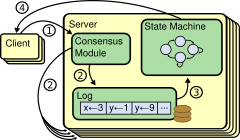
\includegraphics[width=0.5\textwidth, keepaspectratio]{Images/Replicated_state_machine.pdf}
    \caption{Replicated state machine architecture}
    \label{fig:replicated-state-machine}
\end{figure}

Raft implements this replicated log architecture using a collections of servers (a cluster) communicating via remote procedure calls (\textsc{rpc}s), of which there are two: \texttt{appendEntries} and \texttt{requestVote}. At any given time each server is either a \emph{leader}, \emph{follower}, or \emph{candidate} (see \autoref{fig:consensus-fsm}). In normal operation, there is exactly one leader and all other servers are followers.

\begin{figure}[h]
    \centering
    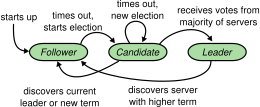
\includegraphics[width=0.5\textwidth, keepaspectratio]{Images/Consensus_FSM.pdf}
    \caption{Server states and the transitions between them}
    \label{fig:consensus-fsm}
\end{figure}

\minisec{Leader election}

A server remains in follower state as long as it receives valid heartbeats (\appendEntriesRPC s that carry no entries) from a leader or candidate. If a follower receives no communication over a period of time, it assumes that there is no viable leader and begins an election to choose a new one. To do so, it transitions to candidate state and issues \requestVoteRPC s in parallel to all other servers in the cluster. Then one of three things happens: (a) the candidate wins the election, (b) another server establishes itself as leader, or (c) a period of time goes by without a winner, in which case a new election is started.

Each server receiving a \requestVoteRPC{} will vote for at most one candidate, on a first-come-first-served basis. Once a candidate wins an election, it becomes the new leader and sends heartbeat messages to every other server to establish its authority.

\minisec{Log replication}

Each client request to a leader contains a command to be executed by the replicated state machines. The leader appends the command to its log as a new entry, then issues \appendEntriesRPC s in parallel to all other servers to replicate the entry. When the entry has been safely replicated, the leader applies the entry to its state machine and returns the result of that execution to the client (for a complete description of what it means for an entry to be \enquote{safely replicated}, see subsection 5.3 of the Raft paper.)

\minisec{Safety guarantees}

In order to guarantee overall correctness, different components of Raft are designed to make sure certain well-defined safety properties are true at all times. These properties are shown to hold and then used to prove correctness in the separate correctness proof \autocite{raftproof}.

Since my project involved changing the way in which quorums\footnote{A \emph{quorum} is a minimal subset of the cluster that an operation has to obtain votes from in order to be performed. Majority voting, for example, specifies that any set of servers containing at least half the servers in the entire cluster constitutes a quorum.} are constructed, I had to pay special attention to the Election Safety property (stating that there can be at most one leader at any given time) and all the steps in the proof to do with quorums, in order to make sure all the desired properties still hold.

\section{Introduction to structured voting schemes\label{ssc:structured-voting-schemes}}

By taking into account the identity of nodes, as opposed to just counting them as in the majority consensus algorithm, we can build \emph{structured} voting schemes.

\minisec{Quorum systems}

A quorum system is defined as a tuple of a read and a write quorum set whose elements are called read quorums and write quorums, respectively. These are constructed such that every write quorum intersects with every other write quorum and with every read quorum in at least one process; read quorums need not intersect \autocite{voting}.

The key realisation that lead to this project was that write quorums have precisely the property required for Raft's leader election, namely that any two write quorums intersect. From this point on, \emph{quorum} will mean \emph{write quorum} unless specifically noted otherwise.

\minisec{Structured voting by example\label{voting-example}}

Structured voting schemes impose a logical structure on the set of processes and use structural properties to specify quorum systems. For example, the structured Grid Protocol arranges processes in a logical rectangular grid \autocite{grid}. A write quorum consists of all processes from a complete column plus one process from each column.

\begin{figure}[h]
    \centering
    {\ttfamily\color{gray}
    \begin{tabular}{c | c | c | c}
        A & \voted{B} & C & D \\
        \hline
        E & \voted{F} & \voted{G} & H \\
        \hline
        \voted{I} & \voted{J} & K & L \\
        \hline
        M & \voted{N} & O & \voted{P} \\
    \end{tabular}
    }
    \caption[Grid protocol quorum table]{A Grid Protocol quorum: The entire second column (\texttt{B}, \texttt{F}, \texttt{J}, \texttt{N}) and one process from each other column (\texttt{I}, \texttt{G}, \texttt{P}) are included}
    \label{fig:grid-quorum}
\end{figure}

\minisec{Specifying voting structures}

\citeauthor{generators} present \emph{tree-shaped voting structures} as a universal quorum system representation in the form of semantics-enriched tree graphs. They are produced by voting structure specific \emph{voting structure generators} \autocite{generators}.

In a tree-shaped voting structure, each node without children (a \enquote{physical node}) represents a process. Nodes with children (called \enquote{virtual nodes}) represent the structure of the voting scheme. The tree is to be interpreted such that votes flow upwards, from the physical nodes (the leaves of the tree) up to the virtual node at its root.

When a physical node casts its vote, its votes are added to the votes its parent virtual node has already received. If the sum of those votes equals or exceeds the parent node's threshold, then the parent node in turn passes its vote to its parent. An annotated example is given in \autoref{fig:majority5-defs}.

\begin{figure}[h]
    \centering
    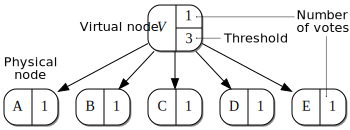
\includegraphics[width=0.6\textwidth, keepaspectratio]{Images/Majority5-defs.pdf}
    \caption[Tree-structured voting scheme for a Majority Protocol]{A tree-structured voting scheme for a Majority Protocol managing five processes.}
    \label{fig:majority5-defs}
\end{figure}

\section{Software engineering\label{sc:software-engineering}}

\subsection{Requirements analysis\label{sc:requirements-analysis}}

\begin{table}[h]
    \centering
    \begin{tabularx}{\textwidth}{X c c}
        \toprule
        \textit{Objective} & \textit{Importance} & \textit{Difficulty} \\
        \midrule
        Voting structure and state type specification & high & medium \\
        Core voting algorithm & high & hard \\
        Voting structure visualiser & medium & medium \\
        Majority Protocol voting structure generator & high & easy \\
        Grid Protocol voting structure generator & medium & hard \\
        Generalised Tree Quorum Protocol voting structure generator & low & hard \\
        Rafter integration & high & hard \\
        Memcached frontend & high & hard \\
        Amazon \ECC benchmark set-up & high & hard \\
        Benchmarking and analysis of the results & high & medium \\
        \bottomrule
    \end{tabularx}
    \caption{Objectives of the project}
    \label{tab:objectives}
\end{table}

\begin{figure}[h]
    \centering
    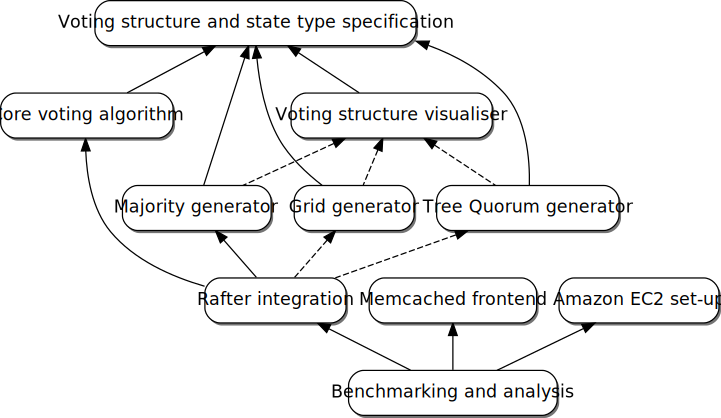
\includegraphics[width=1\textwidth, keepaspectratio]{Images/Dependencies.pdf}
    \caption{Dependency graph of the project's main components. Arrows point from dependent components to their dependencies.}
    \label{fig:dependencies}
\end{figure}

The main software engineering technique I used to increase my chances of success were \emph{modularisation} and \emph{testing} using appropriate measures.

\subsection{Modularisation}

This technique permeated all levels of the project. The code itself was written in a functional style, where each function typically spans between one and ten lines. This increased understandability by forcing me to split larger functions into smaller ones, each performing a small and well-defined task.

All development took place using Git, a popular version control system.\footnote{Git (\url{http://git-scm.com}) is an open source distributed version control system emphasising speed, originally developed by Linux Torvalds to simplify the development of the Linux kernel. Git supports very cheap and fast branching, a feature I used extensively in this project.} I used Git's branching facility to keep independent pieces of code separate during their development. Whenever code from different branches needed to be combined, I merged the required feature branches into a temporary branch. For convenience, all documentation (including the proposal, the progress presentation and this very report) was kept under its own branch in the same repository.

\begin{table}[h]
    \centering
    \begin{tabularx}{\textwidth}{l X}
        \toprule
        \textit{Branch name} & \textit{Description} \\
        \midrule
        \texttt{structured-voting} & Voting algorithms and voting structure generators \\
        \texttt{memcached} & Memcached frontend \\
        \texttt{time-to-consensus} & Time-to-consensus logging \\
        \texttt{failure-command} & Follower failure simulation \\
        \texttt{ec2-integration} & Amazon \ECC instance administration scripts \\
        \bottomrule
    \end{tabularx}
    \caption{Feature branches used in the project repository}
    \label{tab:branches}
\end{table}

The voting algorithm, the voting structure visualiser and the generators for the Majority Protocol and the Grid Protocol were initially written and tested independently from Rafter. Only once I was sufficiently confident in the correctness of the code did I integrate it with Rafter. This integration process turned out to take much less time than expected -- due to the modularity of Rafter, only few changes were required in order for it to use my generalised voting functions.

\subsection{Testing}

In general, I did a lot of manual testing in the early stages of the development of each component. Once the code had reached a stage where testing by hand did not uncover any more bugs, I wrote a QuickCheck test for that component.

Voting structure generators, in particular, were tested using two complementary methods: visually, I checked them for correctness using the voting structure visualiser (see XXX); a QuickCheck property tested for internal integrity.

\begin{table}[h]
    \centering
    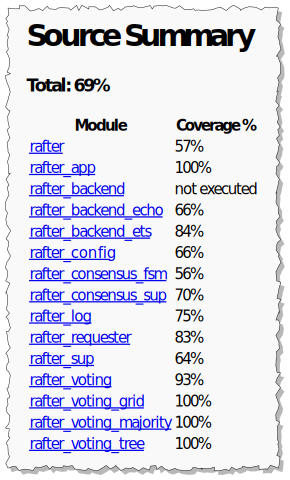
\includegraphics[height=0.45\textheight, keepaspectratio]{Images/Coverage_summary.pdf}
    \caption[Unit test coverage]{Unit test coverage of the structured voting code. Note in particular the high coverage of the last four modules, which were written as part of this project.}
    \label{tab:coverage}
\end{table}

The QuickCheck tests, in their simplest form, consist of \emph{generators} (not to be confused with voting structure generators) and a set of functions specifying the \emph{properties} of the generated objects. QuickCheck then randomly instantiates objects using the generators, and tests if their behave as expected.

\autoref{tab:coverage} shows a screenshot of the test coverage report generated by the EUnit library. I modified four out the five original test modules and added another four to cover my structured voting code. Of the modules shown, I edited \texttt{rafter\_config}, \texttt{rafter\_consensus\_fsm} and \texttt{rafter\_consensus\_sup} and wrote the bottom four modules (all starting with \texttt{rafter\_voting}) from scratch.

\minisec{Generator example}

In \texttt{test/rafter\_gen.erl}, the function \texttt{vstruct()} generates a voting structure, proceeding as follows: It
\begin{inparaenum}[(a)]
    \item creates a list of unique identifiers of random length uniformly distributed between three and 40,
    \item picks a voting structure generator at random (Majority Protocol, Grid Protocol, or Generalised Tree Quorum Protocol),
    \item generates additional parameters depending on the voting structure generator chosen,
    \item calls the chosen voting structure generator with the shuffled list of identifiers and any additional parameters as arguments, and
    \item returns the resulting voting structure.
\end{inparaenum}

This generator function is used wherever a test requires a voting structure. As the tests are run a large number of times, the probability increases that all relevant combinations of parameters are tested at some point.

\minisec{Property example}

The file \texttt{test/rafter\_voting\_majority\_eqc.erl} defines a property of the Majority Protocol in the function \texttt{prop\_majority\_quorum()}. In essence, this property states that an election succeeds if and only if more than half of the nodes agree (\(v \ge \left\lceil n \, / \, 2 \right\rceil \), where \(v\) is the number of votes and \(n\) the total number of processes.)

\section{Implementation approach\label{sc:implementation-strategy}}

XXX

\section{Languages, tools and libraries\label{sc:tools}}

XXX

\subsection{Rafter and structured voting\label{ssc:rafter-structured-voting}}

XXX

In the inception phase of the project, I was faced with the decision of whether to use and existing implementation of Raft or write one from scratch. Since I was primarily interested in implementing structured voting algorithms, and many implementations of Raft already exist, I decided to adapt an existing implementation.

Having written a distributed key-value store in Node.js during an internship, I decided to look for an implementation that used a programming language with built-in support for concurrency that I had heard of: Erlang. Out of the five Raft implementations written in Erlang, Andrew Stone's \emph{Rafter} seemed to be the most mature.\footnote{Andrew Stone is a Distributed Systems Developer at Basho Technologies (\url{http://basho.com}). Rafter is an open source project hosted on GitHub (\url{http://github.com/andrewjstone/rafter}).}

The choice of Erlang and Rafter then dictated my primary programming toolkit:

\begin{description}
    \item[Erlang] A dynamically typed functional programming language originally designed to run Ericsson's telephony switches, Erlang features a run-time system with built-in support for concurrency, distribution and fault tolerance.
    \item[Open Telephony Platform] Commonly referred to as \enquote{the \textsc{otp}}, the Open Telephony Platform provides a set of Erlang libraries and design principles providing middle-ware to develop Erlang applications.
    \item[QuickCheck] A commercial testing framework for Erlang by Quvik \textsc{se}. Rafter's unit and integration tests use it, and I adapted and amended them to cover my code as well.
    \item[Dialyzer] The \enquote{Discrepancy Analyzer for Erlang programs} is used to statically type check Erlang programs.
\end{description}

\subsection{Amazon \ECC and benchmarking\label{ssc:ec2-benchmarking}}

XXX

\section{Summary}

XXX

\chapter{Implementation\label{ch:implementation}}

% \begin{itemize}
    % \item Describe what was actually produced
    % \item Design strategies (looking ahead to the testing stage)
    % \item Draw attention to the parts of the work which are not your own
    % \item Mention major milestones
% \end{itemize}

\section{Overview}

two parts

also: how much of the code is mine? -- \texttt{git diff master --stat src/}

structured voting: Erlang, functional programming

benchmarking: Python, boto, Julia, automatisation and analysis

\subsection{A note on functional programming\label{ssc:fp-note}}

Most of the code written for this project is in Erlang. Being a functional programming language, Erlang supports a very dense programming style. Its core libraries (which are imported by default) include modules for working with lists, dictionaries (hashmaps), sets, string, timers, \textsc{i/o} and databases as well as random values, each of which is used in my code at some point, among others.

Just to illustrate this point, I picked a typical line of Erlang code (\autoref{lst:erlang-majority}) and \enquote{translated} it into relatively idiomatic \textsc{c}++03 (\autoref{lst:cpp-majority}.) Note that the Erlang code only makes use of the built-in module \texttt{dict}, so no imports are required. As a dynamically typed language, Erlang does not need type declarations either, although they \emph{can} be added as annotations to functions for clarity. Thus, the code in \autoref{lst:erlang-majority} really does stand on its own, as long as it is wrapped in a function.

\begin{listing}[h]
    \begin{erlangcode}
NewIndices = dict:map(fun(_, Paths) -> [[0|P] || P <- Paths] end, Indices)
    \end{erlangcode}
    \caption{A typical line of Erlang code, taken from the Grid Protocol voting structure generator. Note how the use of higher-order functions like \texttt{dict:map}, anonymous functions and list comprehensions allows for very dense code.}
    \label{lst:erlang-majority}
\end{listing}

\begin{listing}[h]
    \begin{cppcode}
#include <map>
#include <deque>

typedef int id;
typedef std::deque<std::deque<std::size_t> > paths_t;

// ...

for(std::map<id, paths_t>::iterator indices_it = indices.begin();
        indices_it != indices.end(); ++indices_it) {
    paths_t paths = indices_it->second;
    for(paths_t::iterator paths_it = paths.begin();
            paths_it != paths.end(); ++paths_it) {
        paths_it->push_front(0);
    }
}
    \end{cppcode}
    \caption{The Erlang code from \autoref{lst:erlang-majority}, translated into relatively idiomatic \textsc{c}++.}
    \label{lst:cpp-majority}
\end{listing}

\section{Voting algorithm and data types}

Two data types are used in the structured voting code: one to represent a voting structure, and one to represent the state of an election. Both are implemented as record types in Erlang, and are called \texttt{vstruct} and \texttt{vstate}, respectively; their internal structure is very similar. They are used as follows:

\begin{enumerate}
    \item A voting structure generator creates a \texttt{vstruct}.
    \item This voting structure is used to initialise a new election state \texttt{vstate}.
    \item The election state is updated by the voting algorithm whenever new votes arrive until the election succeeds or fails.
\end{enumerate}

The core voting algorithm as illustrated in \autoref{fig:grid4-state} lends itself well to a recursive implementation.

\begin{figure}[p]
    \centering
    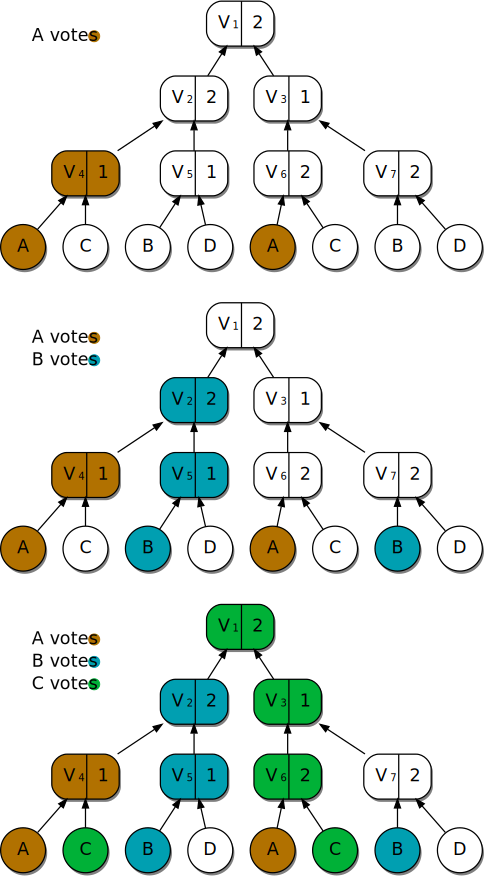
\includegraphics[width=0.9\textwidth, height=0.77\textheight, keepaspectratio]{Images/Grid4-state.pdf}
    \caption[An election using the Grid Protocol]{An election using the Grid Protocol. Each node has one vote. \texttt{A} votes first (maroon). \(V_4\) has a threshold of one, so it votes as well. \(V_2\) and \(V_6\) both have threshold two, so their votes are pending. Then \texttt{B} votes (blue), triggering a vote from \(V_5\). Now both \(V_4\) and \(V_5\) have voted, so \(V_2\)'s threshold of two is reached and it votes, too. At this stage, \(V_1\) and \(V_7\) each require one more vote. Lastly, \texttt{C} votes (green). \(V_4\) has already voted, so nothing happens in this branch. \(V_6\) receives a second vote, so it passes its vote to \(V_3\), immediately triggering it to vote to the root node \(V_1\), where the threshold is now reached, ending the election.}
    \label{fig:grid4-state}
\end{figure}

XXX

\section{Voting structure generators}

In this section, I will describe how the voting structure generators for the three voting protocols I implemented work. These generators output tree-shaped voting structures, which are universal in expressing quorum systems \autocite{structures}. The challenge in building them is to translate the protocol specifications into tree-shaped voting structures.

To simplify this translation, I will now introduce two common patterns that will be used in the description of the Grid Protocol and the (Generalised) Tree Quorum Protocol: \emph{any}- and \emph{all}-nodes.\footnote{Note that the terms any-node and all-node are not used in structured voting literature, but I found them very helpful when designing or reading voting structures.}

\begin{figure}[h]
    \centering
    \begin{subfigure}[t]{0.4\textwidth}
        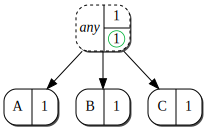
\includegraphics[width=\textwidth, keepaspectratio]{Images/Any.pdf}
        \caption{An any-node has a threshold of one, so it votes as soon as \emph{any} of its children do.}
        \label{fig:any}
    \end{subfigure}
    \quad
    \begin{subfigure}[t]{0.4\textwidth}
        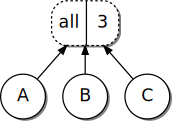
\includegraphics[width=\textwidth, keepaspectratio]{Images/All.pdf}
        \caption{An all-node's threshold is equal to the number of children it has, so it requires \emph{all} of them to vote.}
        \label{fig:all}
    \end{subfigure}
    \caption{Common patterns in tree-shaped voting structures.}
    \label{fig:tsvs-patterns}
\end{figure}

Any-nodes have a threshold of one. This means that they pass their vote to their parent as soon as any of their children vote. In logical terms, any-nodes express a logical \emph{or}: In \autoref{fig:any}, the root votes if and only if \texttt{A} \emph{or} \texttt{B} \emph{or} \texttt{C} vote. More formally, if for a process \(p\), \(p = \text{true}\) denotes that \(p\) votes,

\[ \text{any-node} = \bigvee_{p\,\in\,\text{Children}(\text{any-node})} p \]

In contrast, all-nodes have a threshold equal to the number of children they have, so they vote when all their children have voted. In this sense, all-nodes are the tree-shaped voting structure equivalent of the logical \emph{and}: The root in \autoref{fig:all} votes if and only if \texttt{A} \emph{and} \texttt{B} \emph{and} \texttt{C} vote. Taking the same mapping between truth assignments and voting as above,

\[ \text{all-node} = \bigwedge_{p\,\in\,\text{Children}(\text{any-node})} p \]

In the following, \(n\) refers to the total number of processes.

\subsection{Majority Protocol}

The Majority Protocol (also know as Majority Consensus Voting\autocite{majority}) requires quorums to contain \(\left\lceil (n + 1) / 2 \right\rceil\) processes. This makes it an unstructured voting protocol. However, unstructured voting protocols can be regarded as a subclass of structured voting protocols, since they fit into the same framework of voting structure generators.

\begin{figure}[h]
    \centering
    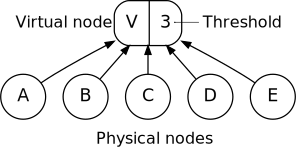
\includegraphics[width=0.5\textwidth, keepaspectratio]{Images/Majority5.pdf}
    \caption{Voting structure for the Majority Protocol with five processes.}
    \label{fig:majority5-struct}
\end{figure}

This voting structure has a rigid format, which allows for a straightforward implementation: It consists of \(n\) physical nodes, all sharing the same virtual parent node (which also acts as the root of the tree-shaped voting structure). Each physical node has one vote, and the threshold of the root node is \(\left\lceil (n + 1) / 2 \right\rceil\). An example for a Majority Protocol voting structure with five processes and a corresponding threshold of three is given in \autoref{fig:majority5-struct}.

\subsection{Grid Protocol}

The Grid Protocol was introduced in the Preparation chapter as an example (see \autoref{voting-example}). It arranges processes in a logical rectangular grid \autocite{grid}; a quorum consists of all processes from a complete column plus one process from each column.

Assuming for now that our nodes fit into a rectangular \(c \times r\) grid so that \(n = c r\) we can translate the requirements of this specification into a voting structure as follows:

\begin{description}
    \item[\enquote{all processes from a complete column}] This means that there must be one column such that every process in that column has voted. The literature calls this the \textsc{cc}-cover, for \emph{complete column cover}. In logical terms, it can be expressed as \(\bigvee_c \bigwedge_{p\,\in\,c} p \), where \(c\) ranges over the columns.

        Using the analogy between logic and tree-shaped voting structures introduced at the beginning of this section, we can translate this formula into a voting substructure as follows: for each column \(c\), there is an all-node whose children are the processes in that column (this models \(\bigwedge_{p\,\in\,c} p \).) The root of the substructure is an any-node, which has the all-nodes as its children. It is the \enquote{\textsc{cc}-cover subroot} in \autoref{fig:grid4-covers}.

    \item[\enquote{one process from each column}] Translating this requirement (called \textsc{c}-cover for \emph{column cover}) into logic, we have \(\bigwedge_c \bigvee_{p\,\in\,c} p \).

        We model this expression as a tree-shaped voting structure as follows: for each column \(c\), we add an any-node whose children are the processes in that column (giving us \(\bigvee_{p\,\in\,c} p \).) These any-nodes are given an all-node as their parent, called \enquote{\textsc{c}-cover subroot} in \autoref{fig:grid4-covers}.
\end{description}

\begin{figure}[h]
    \centering
    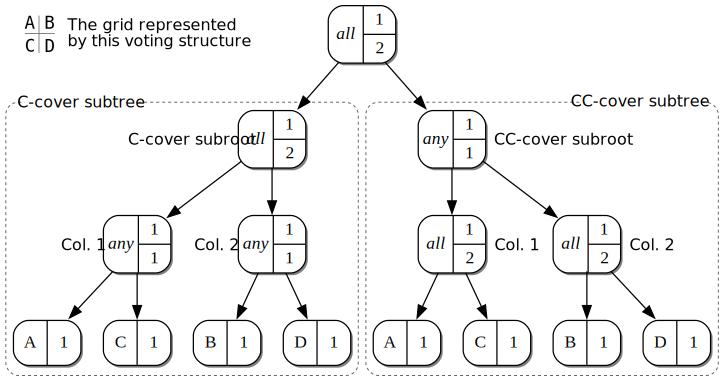
\includegraphics[width=\textwidth, keepaspectratio]{Images/Grid4-covers.pdf}
    \caption{Annotated voting structure for the Grid Protocol with four processes.}
    \label{fig:grid4-covers}
\end{figure}

The Grid Protocol specification demands that both requirements must be fulfilled in order to reach a quorum. We thus make the \textsc{cc}-cover root and the \textsc{c}-cover root the children of an all-node as in \autoref{fig:grid4-covers}, giving \( \left[ \bigwedge_c \bigvee_{p\,\in\,c} p \right] \wedge \left[ \bigvee_c \bigwedge_{p\,\in\,c} p \right] \) as required -- note how the tree-shaped voting structure resembles the abstract syntax tree of the logical expression. This makes sure that an election only succeeds when both a \textsc{cc}-cover and a \textsc{c}-cover have been found.

\minisec{Dealing with incomplete grids}

In the description of the Grid Protocol above, we assumed that the number of processes \(n\) fits nicely into a rectangular grid with \(r\) rows and \(c\) columns. We can of course always enforce this, even when the number of processes is prime, by letting either \(r = 1\) or \(c = 1\). In these extreme cases, however, the Grid Protocol reduces to locking \emph{all} processes:

\begin{description}
    \item[\(\mathbf{r = 1}\)] makes the \textsc{c}-cover equal to the set of all nodes;
    \item[\(\mathbf{c = 1}\)] makes the \textsc{cc}-cover equal to the set of all nodes.
\end{description}

This is clearly not desirable. Instead, the grid structure we impose on the processes is the smallest almost-square grid that all processes can fit in.\footnote{Almost-square here means that \(c\) and \(r\) differ by at most one, so \(|\,c - r\,| \leq 1\).} Specifically, we let

\[ (r, c) =
    \begin{cases}
        \;\left( \left\lceil \sqrt{n} \right\rceil,
                 \left\lfloor \sqrt{n} \right\rfloor \right)
                 & \text{if } \left\lceil \sqrt{n} \right\rceil
                        \cdot \left\lfloor \sqrt{n} \right\rfloor \geq n \\[0.5em]
        \;\left( \left\lceil \sqrt{n} \right\rceil,
                 \left\lceil \sqrt{n} \right\rceil \right) & \text{otherwise}
    \end{cases}
\]

Note that this implies \(r \geq c\); we are said to be \enquote{favouring rows}. Swapping \(r\) and \(c\) on the left-hand side lets us construct grids \enquote{favouring columns}.

The slots in the grid that are not taken up by a process are then considered to be populated by dead placeholder processes. As a little optimisation, we can remove the \textsc{cc}-covers for the columns that contain a placeholder since those columns can never be complete.

\subsection{(Generalised) Tree Quorum Protocol}

The Tree Quorum Protocol \autocite{tree} comes in many flavours which allows for different trade-offs between read and write quorum size to be made. For my voting structure generator, I picked the variant with the smallest write quorum called \enquote{log write protocol} since read quorums are not used in this project.

In this protocol, the processes are logically arranged in a tree of degree \(d\) (meaning that every parent has \(d\) children). For now, we assume that the tree is complete, that is, it has the maximum number of nodes. A quorum is then defined as any set of nodes forming a path from the root to any leaf of the tree.

\begin{figure}[h]
    \centering
    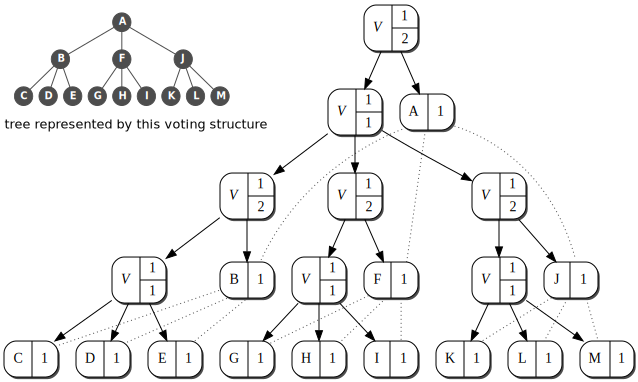
\includegraphics[width=0.9\textwidth, keepaspectratio]{Images/Tree3_13.pdf}
    \caption{Voting structure for the Tree Quorum Protocol based on a ternary tree with 13 processes. Processes \texttt{A}, \texttt{F} and \texttt{G} have voted. They lie on a path from the root (\texttt{A}) to a leaf (\texttt{G}), so they form a quorum. The dotted grey lines are not part of the voting structure proper; they only indicate how the original tree is preserved in the voting structure.}
    \label{fig:grid3_13}
\end{figure}

Take the tree in the top left-hand corner of \autoref{fig:grid3_13} as an example. Building the voting structure bottom-up, we start by assembling a substructure representing the subtree with root \texttt{B}. This substructure should only vote if \texttt{B} and one of \texttt{C}, \texttt{D} or \texttt{E} have voted: \( \texttt{B} \wedge \bigvee_{p\,\in\,\text{Children}(\texttt{B})} p \). We can model this easily in terms of any-nodes and all-nodes: \texttt{C}, \texttt{D} and \texttt{E} are given an any-node as their parent, and this any-node and \texttt{B} are made the children of an all-node.

We proceed in the same way for the subtrees rooted in \texttt{F} and \texttt{J}, and then for the entire tree with \texttt{A} at its root and \texttt{B}, \texttt{F} and \texttt{J} as its children. Note that this is the only truly recursive tree-shaped voting structure: Majority Protocol voting structures always have a height of two, and any Grid Protocol voting structure is four nodes high. Tree Quorum voting structures, on the other hand, have height \(\log_d{n+1}\) (this is a natural number assuming that the trees are always complete.)

\minisec{Dealing with incomplete trees}

Considering incomplete trees leads us from the Tree Quorum Protocol \autocite{tree} to the Generalised Tree Quorum Protocol \autocite{gen-tree}. In the special case of the \enquote{log write} protocol, however, there is no difference in the algorithm: a quorum still consists of a path from the root to a leaf.

XXX more explanation required? side-by-side diagrams?

\section{Integration with Rafter}

Having written and tested the structured voting code, I integrated it into Rafter. This process took place in rougly the following steps:

\begin{enumerate}
    \item Integrating my code with Rafter meant reading and understanding its source code first: 1,500 lines of code,\footnote{That's 1,500 actual lines of code as measured by \texttt{cloc} (\url{http://cloc.sourceforge.net}). See \autoref{ssc:fp-note} for a discussion of Erlang's code density.} spread over 11 modules and undocumented except for a few comments, in a language I was still learning. Using module and function names as a guide, I found the relevant pieces of code that needed changing. Andrew Stone, the developer of Rafter, helped me understand the purpose of a few functions whose task I could not figure out myself.
    \item I renamed my modules and moved them into the appropriate directory to fit into the naming scheme and directory structure of Rafter. Also, the type specifications had to be pasted into the appropriate include file.
    \item In order to use my structured voting code, the node configuration had to be changed from a list of peers (which is all that is needed when only the Majority Protocol is used) to a voting structure (enabling Rafter to use other protocols as well.) This required updating every line of code that made use of this field from the configuration record.
    \item All the places in the code which implicitely assumed that the Majority Protocol was being used had to be rewritten. In most cases, this meant making them wrappers around my generalised structured voting code.
\end{enumerate}


\section{Overview of the benchmarking code}

XXX

\section{Memcached frontend}

XXX need to rework this: make it clearer, maybe using a diagram with client, tcp connection to leader, backend etc.?

Memcached is a high-performance key-value cache designed to sit between an application and a database. If the application issues a query that has been seen before by Memcached, it is served from the cache; otherwise, it is executed on the database and the result stored in Memcached. Originally developed for LiveJournal, Memcached is now used by Youtube, Twitter, Reddit, Facebook and Wikipedia, among others.

My implementation of a Memcached frontend for Rafter amounts to a slight abuse of Memcached for my own intentions. First and foremost, Memcached caches are designed to be very fast, at the expense even of durability: clients cannot, in general, expect the cache to keep a value in memory indefinitely -- dropping a key-value pair to make place for a new one is perfectly acceptable for a cache like Memcached. Rafter, in contrast, is designed to be durable: every write operation is flushed to disk at once. Therefore, building a Memcached server on top of it results in an implementation that is orders of magnitude times slower than original Memcached.

I added a Memcached frontend to Rafter for two reasons: to showcase a useful application that could be built on top of it, and to be able to use Memcached's benchmarking tool, \texttt{memaslap}.\footnote{\texttt{memaslap} is part of libMemcached (\url{http://libmemcached.org/libMemcached.html}), an open source library and toolset for Memcached.}

Newer versions of Memcached support a binary protocol,\footnote{Memcached's new binary protocol is described in this document: \url{https://code.google.com/p/memcached/wiki/BinaryProtocolRevamped}.} which I found less ambiguous than the standard text-based protocol. Decoding and encoding binary protocols being a particular strength of Erlang, the decision over which protocol to implement was easy. \autoref{lst:request-header} shows part of the code the implements the decoding of a Memcached request.

Next, I picked the commands and features I wanted the frontend to support. Since it was meant to be a proof-of-concept, I decided to stick to the minimal set of commands required for a key-value store: \texttt{get}, \texttt{set}, and \texttt{noop}, with the obvious meaning. For simplicity, I also decided not to support the data version check feature (the \textsc{cas} header field.)

\minisec{Implementing Memcached}

The actual implementation of the Memcached frontend consists of three parts: A supervisor, protocol decoder/encoder, and a backend.

\begin{description}
    \item[The supervisor] starts and watches over instances of the decoder/encoder. \emph{Supervisors} are a \emph{behaviour} defined in the \textsc{otp}, Erlang's set of core libraries. Crucially, they are notified when a process started by them fails. By default, the Memcached supervisor starts 20 instances of the decoder/encoder, which allows up to 20 clients to connect to the server simultaneously. Whenever one of them crashes, a new decoder/encoder is brought up.
    \item[The protocol decoder and encoder] makes up the actual \enquote{frontend}: this is the component a Memcached client talks to directly via \textsc{tcp}.
    \item[The backend] finally executes the commands decoded by the frontend by reading from and writing to a local database. In Raft terminology, this module constitutes the \emph{state machine}. It uses Erlang's built-in \texttt{ets} (Erlang Term Storage) module for storing the data.
\end{description}

\begin{figure}[p]
    \centering
    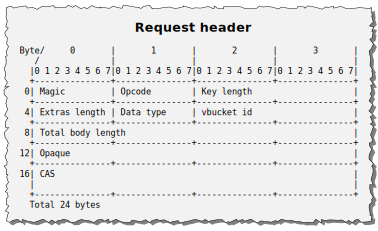
\includegraphics[width=0.7\textwidth, keepaspectratio]{Images/Request_header.pdf}
    \caption[Request header format in Memcached's revamped binary protocol]{Request header format in Memcached's revamped binary protocol. This diagram was taken from screenshot of \url{https://code.google.com/p/memcached/wiki/BinaryProtocolRevamped}.}
    \label{fig:request-header}
\end{figure}

\begin{listing}[p]
    \begin{erlangcode}
case Packet of
    <<_Magic:8,    Opcode:8,    KeyLen:16,
      ExtrasLen:8, _DataType:8, _BucketId:16,
      BodyLen:32,
      Opaque:4/binary,     % binary: 4 bytes = 32 bits
      _CAS:64,             % request header ends here
      Body:BodyLen/binary, % request body
      Next/binary          % start of next request header
      >> ->
      case {Opcode, ExtrasLen, Body} of
          {10, 0, <<>>} ->
              %% NOOP handling
          { 0, 0, <<Key:KeyLen/binary>>} ->
              %% GET handling
          { 1, 8, <<Flags:4/binary, Expiry:32, Key:KeyLen/binary,
                    Value/binary>>} ->
              %% SET handling
      end
    \end{erlangcode}
    \caption[Request decoding in Erlang]{This listing shows the relevant part of the function which decodes Memcached requests from the binary protocol described in \autoref{fig:request-header}. The structure of the \texttt{case Packet of} statement reflects the structure of the packet header. Note how we can use the variable \texttt{BodyLen} captured in the case statement to specify the size of the \texttt{Body} variable within the same case statement. Variables preceded by an underscore are not used.}
    \label{lst:request-header}
\end{listing}

\section{Failure simulation}

XXX

\section{Benchmarking scripts}

XXX

\section{Summary}

XXX

\chapter{Evaluation\label{ch:evaluation}}

% \begin{itemize}
    % \item Signs of success, evidence of thorough and systematic testing
    % \item Sample output, graphs, diagrams
    % \item Original goals achieved? Proof? Did stuff work?
% \end{itemize}

% \begin{itemize}
    % \item Failure modes presentation: most frequent failure modes are individual, then rack failures
% \end{itemize}

\section{Summary}

XXX

\chapter{Conclusions\label{ch:conclusions}}

% \begin{itemize}
    % \item Refer to Introduction
    % \item Lessons learnt
% \end{itemize}

%TC:ignore

\printbibliography

% \backmatter

\appendix

\chapter{Code samples\label{ch:code-samples}}

% \listoffigures
%
% \listoftables
%
% \listofalgorithms

%TC:endignore

\end{document}
